\begin{savequote}[8cm]
It's simple mathematics.
  \qauthor{--- Mos Def, "Mathematics"}
\end{savequote}

\chapter{\label{ch:5-epcoupling}Results II: Electron-phonon and phonon-phonon coupling}
% see ziman electrons and phonons?
% https://journals.aps.org/rmp/pdf/10.1103/RevModPhys.89.015003
\section{Introduction} \label{ch5:introduction}

% simplest approximation is that there is no coupling. But then mobility too large. In reality scattering (see previous chapter)
%include v. brief overview of what each is and explain that it is linked to non-radiative recombination and other important processes, thermal transport.
In the simplest approximation of a semiconductor, a single electron in a perfect lattice at zero kelvin, electrons do not scatter and have infinite mobility. In the next best approximation, we introduce harmonic phonons. The electrons scatter from the phonons and the electron mobility becomes finite. This electron-phonon interaction underpins many phenomena in condensed matter physics and materials science including carrier mobility (as explored briefly in the previous chapter, Section \ref{}), polaron formation (Section \ref{}), hot carrier thermalisation (Section \ref{}) and non-radiative recombination (Section \ref{}). Still, in the harmonic approximation, the phonons do not interact with one another - they have an infinite lifetime. To calculate thermal conductivity or understand how a polaron cools to equilibrium (Section \ref{}) we need to consider anharmonic phonon-phonon interactions. Some processes, such as non-radiative recombination, include electron-phonon and phonon-phonon interactions (Figure \ref{nrr}).

This chapter begins with an introduction to electron-phonon coupling, polaron formation (a result of electron-phonon coupling in an ionic lattice) and phonon-phonon coupling. I have included brief discussion of our understanding of these interactions in hybrid halide perovskites at suitable points.

\begin{figure*}
\includegraphics[width=1.0\columnwidth]{./figures/ch5/epcoupling.png}
\caption[Quasi-particle interactions during non-radiative recombination]{
}
\label{nrr}
\end{figure*}

% Can measure a temperature dependance in the electronic structure:, Peaks shift, Peaks broaden (shorter electron lifetime), There is a direct and indirect (through the change in volume) contribution to dE/DT. , For direct: See AHC theory., For the indirect what we are asking is the effect of thermal expansion. See monserrat work or Bi2Se3 where it is not negligible. For Si the expansion is negligible (Xavier Gonze)

\subsection{Electron-phonon coupling}
To include the effect of electron-phonon interactions we must include a previously ignored term to the system Hamiltonian.
\begin{equation} \label{HamiltonianEP}
    
\end{equation}
The first two terms describe the separate electron and phonon sub-systems, as seen in Section \ref{}. The third term describes the electron-phonon interaction. The electron has an energy eigenvalue $\epsilon$, determined by the crystal momentum $k$ and band $n$. This electron is interacting with a phonon of vibrational frequency $\omega$  , determined by crystal momentum $q$ and branch $v$. The matrix element $g$ determines the strength of the coupling. 


\textbf{Acoustic deformation potential scattering}
Unfortunately Equation \ref{HamiltonianEP} does not tell us how to calculate the coupling term $g$. In 1950 Bardeen and Shockley introduced the `deformation potential' method \cite{}, which gives an approximation to $g$ for semiconductors where the dominant electron-phonon scattering mechanisms involve long wavelength acoustic phonons.\cite{Giustino2016} In this approach $g$ is given by:
\begin{equation} \label{couplingterm}
   q_{mnv}(k,q) = \i\left(\frac{\hbar}{2N_pM_k\omega_{qv}}\right)^{\frac{1}{2}}q\cdot e_{kv}(q) \Omega\frac{\partial\epsilon_{nk}}{\partial\Omega},
\end{equation}
where $N_p$ the number of cells in the supercell, $M_k$ is the mass of the $k$^{th} supercell and \textbf{e}_{kv} is the polarization of the phonon. 

The deformation potential $\Omega\frac{\partial\epsilon_{nk}}{\partial\Omega}$ in Equation \ref{couplingterm} can be determined empirically or calculated from first principles using DFT. There are two ways to do the latter; via density-funtional perturbation theory, or using the `frozen-phonon' approach. The results here use the latter; the energy of the valence and conduction bands are tracked as the crystal lattice is distorted along a single phonon mode. 
%The coupling term $g$ is given by 
%\begin{equation}
%    q_{mnv}(k,q) = \langleu_{mK=q}|\Delta_{qv}v^{KS}|u_{nk}\rangle_{uc}
%\end{equation}

\textbf{Frolich interactions}
For Frolich interactions, the electrons are affected by the electric field generated by longitudinal optical (LO) phonons.
This interaction is available only in ionic crystals, where atomic displacements generate long-range electric fields. In the Frolich model a single electron interacts with the polarization field of an ionic lattice.\cite{Giustino2016}
In this model the effective potential is replaced with
\begin{equation}
    V_0 = \left[\frac{e^2M_k\omega^2_{qv}}{\epsilon_0\Omega}\left(\frac{1}{\epsilon^{\infty}}-\frac{1}{\epsilon^0}\right)\right]^{\frac{1}{2}}\frac{1}{|q|^2}
\end{equation}
where $\epsilon_0$,$\epsilon^0$ and $\epsilon^{\infty}$ is the vacuumn static relative and high-frequency relative permittivities respectively.

Electron-phonon interactions are expected to be significant \ce{CH3NH3PbI3} (MAPI) as MAPI is a soft material, with structural distortions and dynamic disorder at room temperature.
Furthermore, long carrier lengths but modest mobilities in MAPI point to strong electron-phonon interactions.\cite{} 
% https://pubs.acs.org/doi/pdf/10.1021/acs.jpclett.5b02390 
Photoluminescence studies of FAPI suggest that acoustic deformation potential scattering makes only a minor contribution to electron-phonon interactions at room temperature, \cite() %  Electron-Phonon Coupling in Hybrid Lead Halide Perovskites.Nat. Commun.2016,7, 11755
whilst electron-phonon coupling is reduced below the temperature correponding to the relevant LO phonon for Frolich coupling. This suggests that Frolich interactions dominate, and is supported by a theoretical calculation which predicts a LO-phonon limited mobility in line with experiment.\cite{Jarv}

% Robert Lobronvnic Optical phonon modes hbarw are occupied at kT @ room temperature: RARE
\subsection{Phonon-phonon coupling}
% can also assume that no phonon-phonon scattering. Infinite lifetimes and conductivity - not the case in MAPI.
% Halide perovskites show unusual cooling kinetics for above bandgap photo-excitation; cooling is slower than that observed in other semiconductors and this has been attributed to a ``hot phonon bottleneck''. This has been described as a two-step process: initial thermalisation, then cooling to equilibrium.

% experimental measures - see summary on github.

%\begin{figure}[h!]
%\centering
%  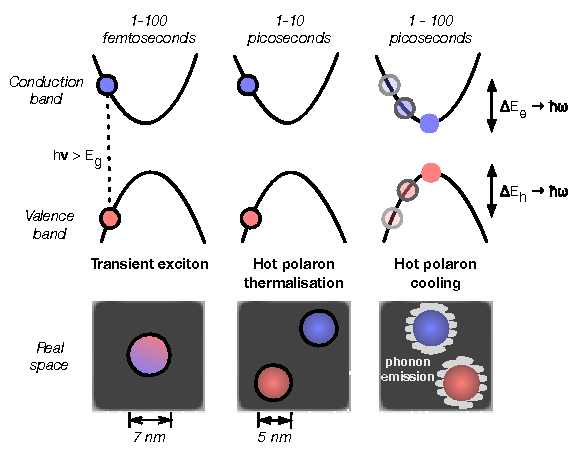
\includegraphics[width=0.7\columnwidth]{C05/figs/f1.pdf}
%  \caption{Reproduced from reference \cite{Whalley2017a}.}
%  \label{cooling_schematic}
%\end{figure}
%\section{Summary}


% in MAPI: short thermal lifetimes
% Low thermal conductivity is linked to material breakdown explains why all of their perovskite LEDs break very quickly (heat builds up and kills the material) - much higher currents than solar cells
% Thermal stability: aron says good article on latest advances: https://pubs.acs.org/doi/10.1021/acs.jpclett.8b00463

% what is happening in this chapter: calculated for MAPI.
% Modes are the soft modes: Anharmonic soft tilting modes are characteristic of the perovskite material family. For cubic perovskite with a unit cell of The tilting corresponds to opposite tilting in neighbour cell, so happens at M (0.5,0,0) amd R (0.5,0.5,0). Hybrid halide perovskites have double-well potentials associated with octahedral tilting of the inorganic lattice. These are located at the $M$ and $R$ point in the brillouin zone.
%We use a `mode mapping' approach to distort the structure along the $M$ and $R$ eigenvectors and track the change in bandgap as a function of the normal mode coordinate $Q$ (which corresponds to the amplitude of the phonon mode).


\section{Methods}
\subsection{Soft mode potential energy surface}
\subsection{The frozen phonon method}
% cite Jonathan repo

% see guistino.

%Bandgaps were computed within the Kohn-Sham density-functional theory (DFT) formalism as implemented in the \textsc{VASP} code\cite{Kresse1996a}.
%The valence wavefunctions were expanded in a plane-wave basis set with a 700 eV cut-off and the exchange and correlation interactions between electrons were modelled using the PBEsol exchange-correlation functional\cite{Perdew2008a} ($Q$ from 0 to 150 amu$^{\frac{1}{2}}$ \AA) and a screened hybrid functional (HSE06)\cite{Heyd2004a,Heyd2005a} ($Q$ from 0 to 69 amu$^{\frac{1}{2}}$ \AA).
%Scalar-relativistic corrections were used for the core electrons within the projector augmented-wave (PAW) formalism,\cite{Blochl1994} with the outermost s and p electrons of C, N and I, and the outermost s, p and d electrons of Pb, being treated as valence. 
%The PAW projection was applied in reciprocal space (\textsc{LREAL = .FALSE.} in \textsc{VASP}).
%Spin-orbit coupling, which strongly affects the unoccupied conduction band, was considered for the PBEsol functional.
%A Monkhorst-Pack \textit{k}-point grid, with a $\Gamma$-centered $6 \times 6 \times 6$ grid, was used to integrate the electronic Brillouin zone.
%A total-energy convergence criterion of $10^{-8}$ eV during the electronic minimisation was found to be necessary to remove noise in the absolute electronic eigenvalues.
%A least-squares polynomial fit using the \textsc{Python} library \textsc{Numpy} was applied to the symmetrised data.

% deep level reference potential
% cite Jarv for EP
\subsection{Frolich polaron model parameters}
% cite Jarvist work
\subsection{Hot carrier cooling rate}


\section{Results}

\subsection{Potential Energy Surface for soft modes}
% Reported elsewhere but included for discussion.% We differentiate between the imaginary modes which result from numerical inprecision and those which can tell us something about the dynamical disorder of the crystal structure
%  A crystal is dynamically stable at equilibrium if atomic displacements increase the potential energy of the system. Within the harmonic approximation, dynamic stability results in real and positive phonon frequencies $\omega$ when solving the eigenvalues of the dynamical matrix $D(\mathbf{q})$, 
%\begin{equation}
%    D(\mathbf{q})\mathbf{e}_{\mathbf{q}j} = \omega^2_{\mathbf{q}j}\mathbf{e}_{\mathbf{q}j}
%\end{equation}
%where $\mathbf{q}$ is the wave vector, $j$ is the band index, $\omega_{\mathbf{q}j}$ and $e_{\mathbf{q}j}$ are the phonon frequency and polarization vector of the phonon mode respectively. However when performing phonon calculations, negative phonon frequencies may arise due to dynamic instabilities in the crystal. These negative frequencies correspond to imaginary modes which indicate that the potential energy of the crystal can be lowered via atomic displacements from the equilibrium structure. Therefore, these imaginary modes can provide useful information about the stability of a crystal and phase transitions.
% tilting: Experimental evidence: https://arxiv.org/pdf/1606.09267.pdf and https://journals.aps.org/prl/abstract/10.1103/PhysRevLett.118.136001 (not just the hybrids). 
%There is dynamic and static tilting. Dynamic tilting at high temperature. Static tilting at lower temperature. At low temperature there is the coexistance of different phases: as demonstrated by the broadening of PL spectra as demonstrated by Herz’ group in Oxford. You would expect the PL broadening to decrease when lowering temperature as the thermal motion decreases.
%Ruoxi paper - common to all perovskites

%\begin{figure}[ht]
%\includegraphics[width=16.3cm]{C05/figs/bandzoomed.png} \label{phonon_dispersion}
%\caption{
%Phonon dispersion showing soft modes at the $M$ and $R$ points. Frequency is measured in THz.
%}
%\end{figure}

\subsection{Single mode bandgap deformation potential}
% T-dependent broadening from IR: Robert Lovrincic

% \begin{table}[ht]
% \caption {Residual sums of squares (RSS) for quadratic and biquadratic fits to the PBEsol data in Fig. \ref{figs1}. A smaller RSS indicates a better fit of the model to the data.}
%  \label{RSS} 
% \begin{tabular}{cccccccccc} 
% \hline  \hline
% \multicolumn{2}{c}{} & \multicolumn{4}{c}{$M$} & \multicolumn{4}{c}{$R$} \\

% \multicolumn{2}{c}{} & $\Delta$VBM & $\Delta$CBM & $\Delta$E$_g$ & & & $\Delta$VBM & $\Delta$CBM & $\Delta$E$_g$ \\
% \hline
% Quadratic & \hspace{5pt} & $4.1 \times 10^{-3}$ & $ 1.1 \times 10^{-2}$ & $3.7 \times 10^{-3}$& \hspace{5pt} & \hspace{5pt}  & $9.8 \times 10^{-3}$& $2.0 \times 10^{-2}$& $3.5 \times 10^{-3}$\\

% Biquadratic & & $3.2 \times 10^{-3}$ & $2.9 \times 10^{-3}$ & $2.0 \times 10^{-5}$ & & &$6.4 \times 10^{-3}$ &$6.0 \times 10^{-3}$ & $6.0 \times 10^{-5}$\\
% \hline \hline
% \end{tabular}
% \end{table}

%We find that the bandgap $E_g(Q)$ is well described as quadratic over small $Q$, but
%required a biquadratic term to reproduce the correct behaviour at large $Q$.
%It is instructive to also decompose the total band gap deformation into separate contributions from the conduction and valence bands 
%(i.e. electron and hole coupling).
%Unfortunately, the electrostatic summations under periodic boundary conditions 
%do not allow for the determination of absolute electron eigenvalues. 
%So to track the change in eigenvalue across calculations we track the change in the valence- 
%and conduction-band energies with respect to reference deep-lying core states, here the Pb 3d. 
%Fitting a quadratic function to the band energies shows the electron-phonon coupling (i.e. the change in the conduction-band energy)
%to be about three times that of the hole (valence band) coupling. 
%A similar band gap deformation is found for the \textit{M} and \textit{R} modes. This indicates that the local tilting dominates the interaction (i.e. the out-of-phase tilting for successive planes in the \textit{R} mode has little additional effect on the gap).

%\begin{figure}[h]
%\includegraphics[width=16.3cm]{C05/figs/fig_s3.png} \label{figs1}
%\caption{
%Energy change ($\Delta$E) as a function of the normal-mode coordinate $Q$ of the valence-band maximum ($\Delta$VBM), conduction-band minimum ($\Delta$CBM), and band gap ($\Delta$E$_g$) obtained from calculations using the PBEsol functional.
%The energies of the band extrema have been referenced to the energy of the Pb 3d core states.
%}
%\end{figure}


\subsubsection{Exchange-correlation functional dependance}
%\begin{figure}[]
%\includegraphics[width=16.3cm]{C05/figs/fig_s4.png} \label{Egtheory}
%\caption{
%Change in band gap ($\Delta E_g$) as a function of the normal-mode coordinate $Q$ obtained with three exchange-correlation treatments used in the electronic-structure calculations, \textit{viz.} PBEsol, PBEsol with spin-orbit coupling (SoC), and HSE06.
%}
%\end{figure}

%\begin{table}[h]
%\caption {Values of the $a$ and $b$ coefficients in the fitted function $E_g = E_0 + aQ^2 + bQ^4 + O(Q^6)$ used to model the band gap deformation potentials evaluated from frozen-phonon calculations using the PBEsol, PBEsol+SoC and HSE06 exchange-correlation functionals.}
%\label{bandgapF}
%\begin{tabular}{ccccccccc} 
%    \hline\hline
%{Mode} & \hspace{5pt} & {} & \hspace{5pt} & {PBEsol} & \hspace{5pt} & {PBEsol+SoC}& \hspace{5pt} & {HSE06}\\ 
%    \hline
%$M$ && $a$ && \num{2.3e-5}     && \num{2.3e-5}       && \num{2.9e-5} \\
%    && $b$ && \num{-3.3e-10}   && \num{-3.6e-10}     && \num{-5.4e-10} \\
%$R$ && $a$ && \num{2.3e-5}     && \num{2.5e-5}       && \num{2.9e-5} \\
%    && $b$ && \num{-3.0e-10}   && \num{-4.3e-10}     && \num{-7.0e-10} \\ 
%    \hline\hline
%\end{tabular}
%\end{table}


%\begin{table}[]
%\caption {
%Valence- and conduction-band deformation potentials relative to the Pb 3d core energy level obtained from frozen-phonon calculations with three exchange-correlation treatments, \textit{viz.} PBEsol, PBEsol with spin-orbit coupling (SoC), and HSE06.
%}
%\begin{tabular}{ccccccccc}
%\hline \hline
%Mode & \hspace{5pt} & & \hspace{5pt} & PBEsol & \hspace{5pt} & PBEsol+SoC & \hspace{5pt} & HSE06 \\
%\hline
%$M$ & & VBM & & $1.61 \times 10^{-5}$ & & $1.55 \times 10^{-5}$ & & $0.97 \times 10^{-5}$ \\
%& & CBM & & $3.88 \times 10^{-5}$ & & $3.68 \times 10^{-5}$ & & $3.66 \times 10^{-5}$ \\ 
%& & $\frac{CBM}{VBM}$ & & 2.14 &  & 2.37 & & 3.77  \vspace{5pt} \\

%$R$ & & VBM & & $1.34 \times 10^{-5}$ & & $1.01 \times 10^{-5}$ & & $1.33 \times 10^{-5}$ \\
%& & CBM & & $3.52 \times 10^{-5}$ & & $3.37 \times 10^{-5}$ & & $3.96 \times 10^{-5}$ \\
%& & $\frac{CBM}{VBM}$ & & 2.63 & & 3.34 & & 2.98 \vspace{5pt} \\ 
%\hline \hline
%\end{tabular}
%\end{table}


\subsubsection{A note on supercell size}

\subsection{Anharmonic electron-phonon interaction}
% - deformation potential theory: see Jarvist blog notes
% - see monserrat: mean value theorem <o>=integral. 
% The method includes quantum nuclear motion, goes beyond the harmonic regime, but only contains the first-order contribution to the electron-phonon coupling of the band-gap deformation. 
% A positive band-gap shift of 36 meV (\textit{R} point phonon) and 28 meV (\textit{M} point phonon) 
% is predicted at T = 300 K.
\subsection{Hot carrier cooling}
% Now move on to consider...

% 

\subsubsection{Polaron formation}
% include initial polaron temperature as a function of energy and radius: T above bulk.

\subsubsection{Initial thermalisation}
%Initial thermalisation involves heat transfer into the optical phonon modes. This is a fast picosecond process enabled by a coupling to the local polar phonon population. This results in an electron polaron with radius 26.8\AA which occupies 360 unit cells of the crystal. The polaron radius is an upper limit as disorder will increase localisation of the charge carrier. Point and extended defects (surfaces, interfaces, dislocations, grain
%boundaries) may localise polarons further.
%Once fully thermalised, the excess above bandgap energy will be shared
%amongst all accessible phonon states within the polaron. 
%We will calculate the temperature of the resulting Fr{\:o}lich polaron, which depends on the polaron volume and specific heat capacity ($C_V$).

%\begin{figure}[h]
%\centering
%  \includegraphics[width=0.7\columnwidth]{C05/figs/f3.png}
%  \caption{Thermalised polaron temperature in MAPI as a function of polaron
%    radius and excitation  energy assuming a bulk value of the heat capacity. 
%    The calculated bulk electron polaron radius
%    of 26.8 \AA  ~ provides an upper bound for polaron size.
%    We take the lattice parameter (6.3 \AA) as a lower bound---below this the
%    continuum large polaron approach is not valid. 
%    We consider excitation from the bandgap to near-UV. 
%    Inset shows detail at larger radii (axes same as main). }
%  \label{TemperatureRadius}
%\end{figure}


%To calculate the polaron temperature in Figure \ref{TemperatureRadius} we assume equipartition of the above bandgap energy between electron and hole. Near-UV excitation at 4eV gives a maximum energy of 1.2eV which can be transferred to the polaron. The heat capacity is calculated from the bulk phonon density of states: summing over the Bose-Einstein occupied phonon modes for MAPI, we find
%a per-unit cell specific heat capacity of \SI{1.25}{\milli\eV\per\K} at
%\SI{300}{\K}. The temperature increases with localisation ($T \propto r^{-3}$) as shown in Figure \ref{TemperatureRadius}. 

\subsubsection{Cooling to equilibrium}
%The polaron will then cool to equilibrium over hundreds of picoseconds. We consider bulk heat diffusion in the low fluence limit where individual photon quanta are absorbed into isolated hot polarons. The polarons then cool by scattering into phonon modes which diffuse away from the polaron. We consider the polaron as a hot sphere in
%a continuum of ambient temperature material, which allows us to calculate temperature as a function of time using the heat diffusion equation. 

%The use of this classical heat diffusion model is motivated by previous work related to phonon-phonon scattering in MAPI. 
%Due to energy and momentum conservation rules, three-phonon scattering is the lowest-order process. 
%We previously\cite{Whalley2016} calculated the three-phonon interaction strengths for
%MAPI and found them to be orders of magnitude stronger than for CdTe and GaAs. 
%The sum of modal contributions, accounting for phonon lifetime, group velocity
%and heat capacity, gives the overall thermal conductivity.\cite{Togo2015}
%In MAPI, the bulk thermal conductivity from a solution of the Boltzmann
%transport equation (in the relaxation time approximation) is extremely low,
%\SI{0.05}{\watt\per\metre\per\K} at \SI{300}{\K}.\cite{Whalley2016} 
%In contrast, the calculated conductivity for GaAs and CdTe is 
%\SI{38}{\watt\per\metre\per\K}
%and
%\SI{9}{\watt\per\metre\per\K},
%respectively. We will show that polaron cooling in MAPI is slow due to the ultra-low thermal conductivity of the perovskite lattice. 

%\begin{figure}[h]
%\centering
%  \includegraphics[width=0.7\columnwidth]{C05/figs/f4.png}
%  \caption{The energy of a large polaron state (starting at 1.2 eV above the conduction band minimum, with a polaron radius of 26.8 \AA) 
%  in \ce{CH3NH3PbI3} as a function of time.
%  The slow rate is due to the low thermal conductivity in MAPI ($\kappa$ = 0.05Wm$^{-1}$K$^{-1}$). 
%  For comparison, we show the behaviour using the thermal conductivities of 
%  CdTe ($\kappa$ = 9) and GaAs ($\kappa$ = 38). }
%  \label{TemperatureTime}
%\end{figure}

%The polaron is modelled as a hot sphere which reduces the problem to one dimension.
%The initial `top hat' heat distribution is convolved with a Gaussian kernel to
%give an analytical expression for the evolution of hot carrier energy with time (shown
%in Figure \ref{TemperatureTime}).
%The rate of cooling is determined by the diffusivity ($D$): 
%\begin{equation}
%    D= \frac{\kappa}{\rho c_p}
%\end{equation} 
%where $\kappa$ is the thermal conductivity, $\rho$ is the density and $c_p$ is the specific heat capacity. 
%
%Heat diffuses from MAPI on the order of 100 ps, whilst for other conductivities 
%  the process is much faster, on the order of 100 fs. 
%  This is in agreement with reported experimental values: Refs. \cite{Klein2016} (MAPI), \cite{Zhong2017} (CdTe) and \cite{Rosenwaks1993} (GaAs). 
%  Note that at short timescales, measurements of hot carrier cooling in MAPI and \ce{CsPbI3}($\kappa$ = 0.5) may appear linear due to the slower exponential decay.

\section{Summary}

We have shown how Fr{\:o}lich polaron theory and a classical heat diffusion model can be combined to
describe the physical process behind the slow hot-carrier cooling rates
observed for halide perovskites.

\textbf{Data Access Statement}

The crystal structures and phonon data are available at \url{https://github.com/WMD-group/Phonons}. 
and can be processed using the \textsc{Phonopy} packages available from \url{http://atztogo.github.io/phonopy} 

Data files and Jupyter notebooks outlining the calculation steps are available as a repository on GitHub at https://github.com/WMD-group/hot-carrier-cooling.
\textbf{Acknowledgements}
Via our membership of the UK's HEC Materials Chemistry Consortium, which is funded by EPSRC (EP/L000202), this work used the ARCHER UK National Supercomputing Service (http://www.archer.ac.uk).
Calculations were performed on the SiSu supercomputer at the IT Center for Science (CSC), Finland, via the Partnership for Advanced Computing in Europe (PRACE) project no. 13DECI0317/IsoSwitch. We also made use of the Balena HPC facility at the University of Bath, which is maintained by Bath University Computing Services.


